\documentclass[12pt]{exam}

\usepackage{amssymb,amsfonts,amsmath}
\usepackage[letterpaper,margin=1in]{geometry}
\usepackage{graphicx}

\newcommand{\class}{MATH 375}
\newcommand{\term}{Spring 2015}
\newcommand{\doctitle}{Homework 4}

\newcommand{\matlab}{{\sc Matlab}}

\parindent 0ex

\pagestyle{head}
\header{\bf \class}{\bf \doctitle\ - Page \thepage\ of \numpages}{\bf \term}
\headrule

\renewcommand{\arraystretch}{1.5}

\begin{document}

Remember to adequately label all plots and include any \matlab~scripts and functions with your solutions. A clear and complete presentation of your solutions is required for full credit.
\begin{questions}

\question Write a \matlab~function with the declaration \verb$function cobweb(g,a,b,x0,kmax)$ that plots the function \verb$g$ on the interval $[\verb$a$,\verb$b$]$ along with the cobweb diagram showing \verb$kmax$ fixed point iterations of \verb$g$ starting at \verb$x0$. Examples of the function output are shown in Figures \ref{fig:cobweb} and \ref{fig:cobweb2}. Turn in the code for your function and perform or answer the following.

\begin{parts}
\part Use your function to plot the cobweb diagrams for $g_1(x) = \cos(x)$ and $g_2(x) = \cos(x)+2$ starting with any points of your choice.
\part Explain why both iterations must converge if $x_0$ is sufficiently close to the fixed point.
\part Do you observe a difference between the convergence rates for $g_1$ and $g_2$? Explain.
\part Do you expect the iterations for $g_1$ and $g_2$ to be globally convergent? Explain.
\end{parts}

\question Sauer, Section 1.4, Exercise 8.

\question Sauer, Section 1.4, Computer Problem 9.

\question Consider the four-bar planar linkage $ABCD$ shown in the Figure \ref{fig:linkage}, where the four rods have lengths $AB=a_1 =10$,
$BC=a_2 =2$, $CD=a_3 =7$, and $DA=a_4 =6$. This is a planar linkage system, and it can exist in various shapes. Variation of the angle $\alpha$ results in variation of the angle $\beta$, with the two angles related by
\[\frac{a_1}{a_2} \cos\beta - \frac{a_1}{a_4}\cos\alpha - \cos(\beta-\alpha) = - \frac{a_1^2 + a_2^2 - a_3^2+a_4^2}{2\,a_2a_4} .\]
Use the Newton iteration to solve this problem for $\alpha \in [0, 2\pi]$ to a tolerance of $10^{-6}$. For this arrangement and for each value of $\alpha$ in the given range, there are two possible values of $\beta$. Use an initial value $\beta_0 = -\pi/2$ for $\beta$ to ensure that you get $\beta$ in the same contiguous range. Plot the position-dependent midpoint of rod $a_3$ as $\alpha$ takes values in the interval $[0, 2\pi]$.

\begin{figure}[b]
\centering
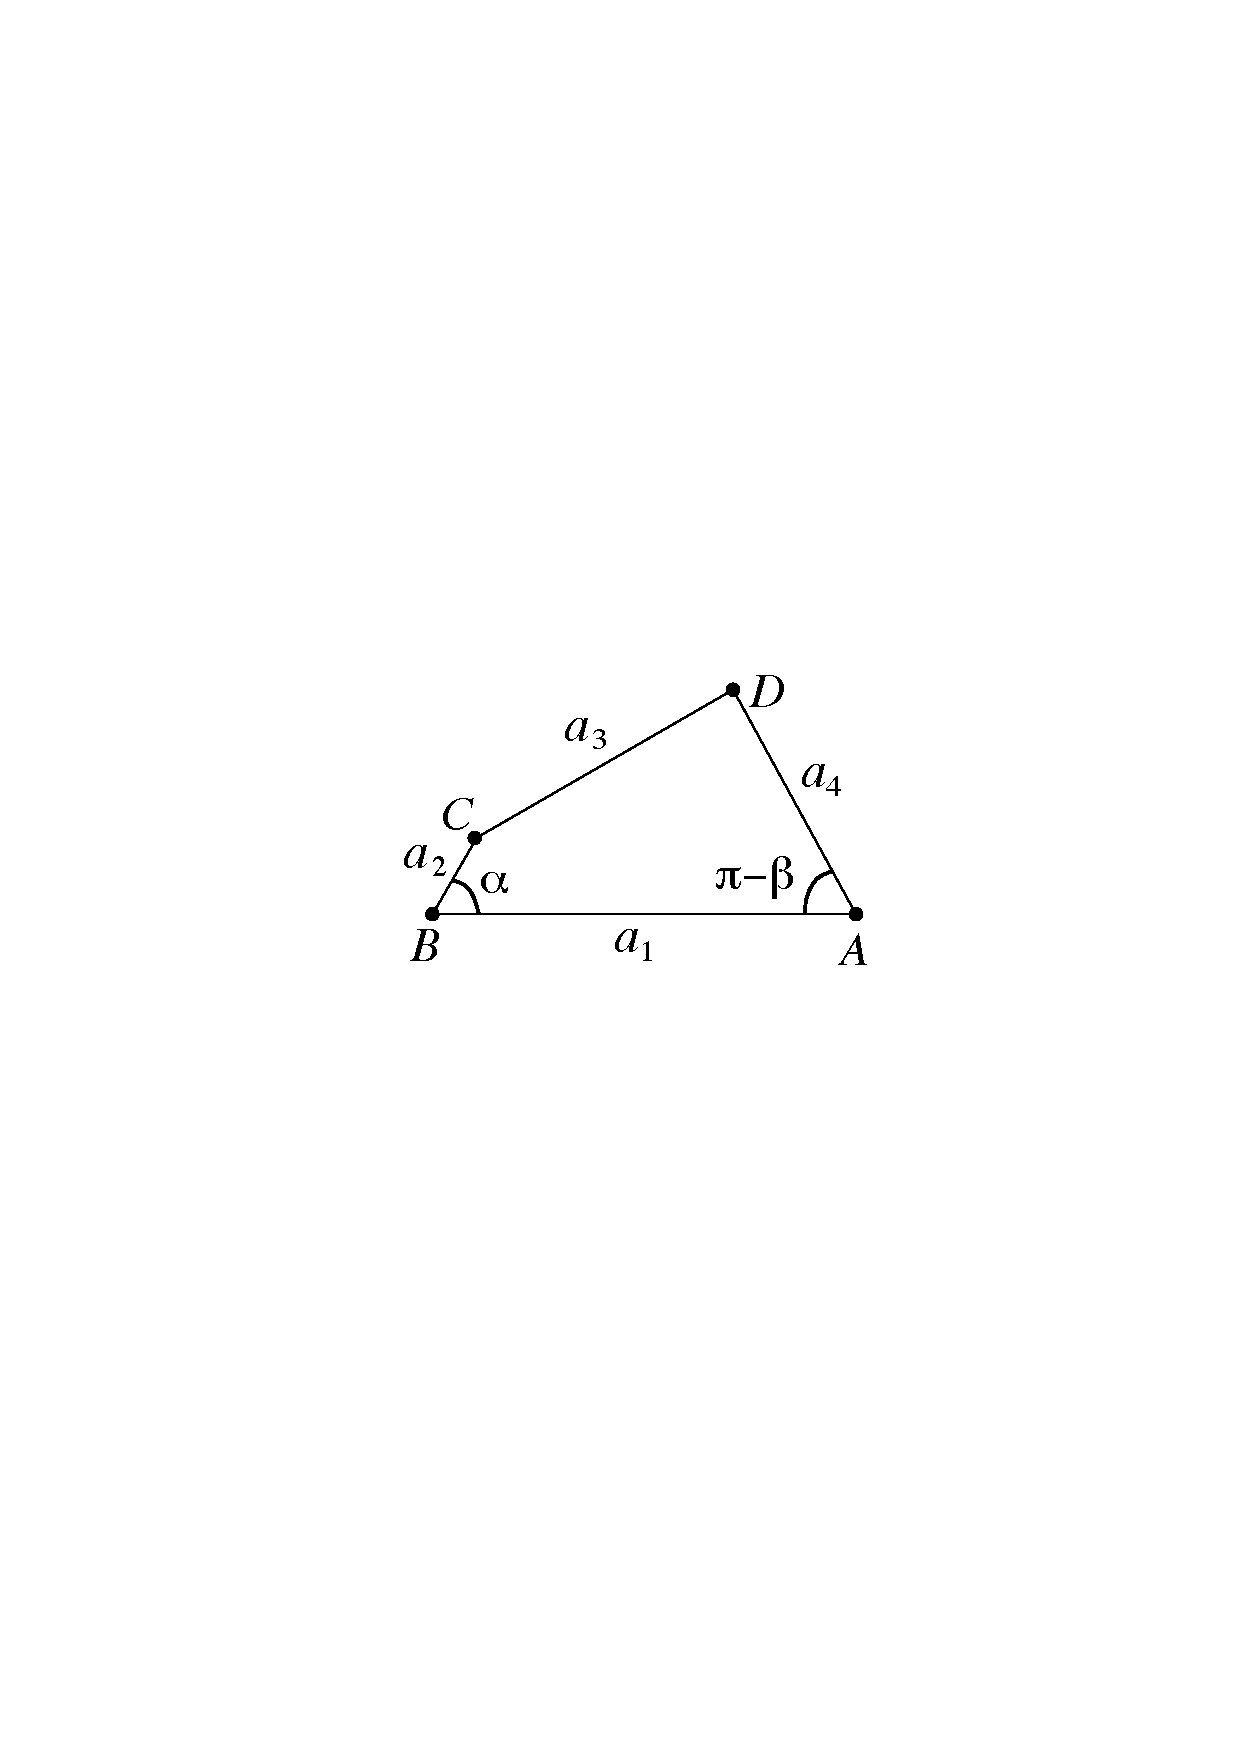
\includegraphics[width=0.4\textwidth]{linkage.pdf}
\caption{A four-bar planar linkage. The bottom bar $a_1$ remains fixed, but all joints are flexible.}\label{fig:linkage}
\end{figure}

\begin{figure}[p]
\centering
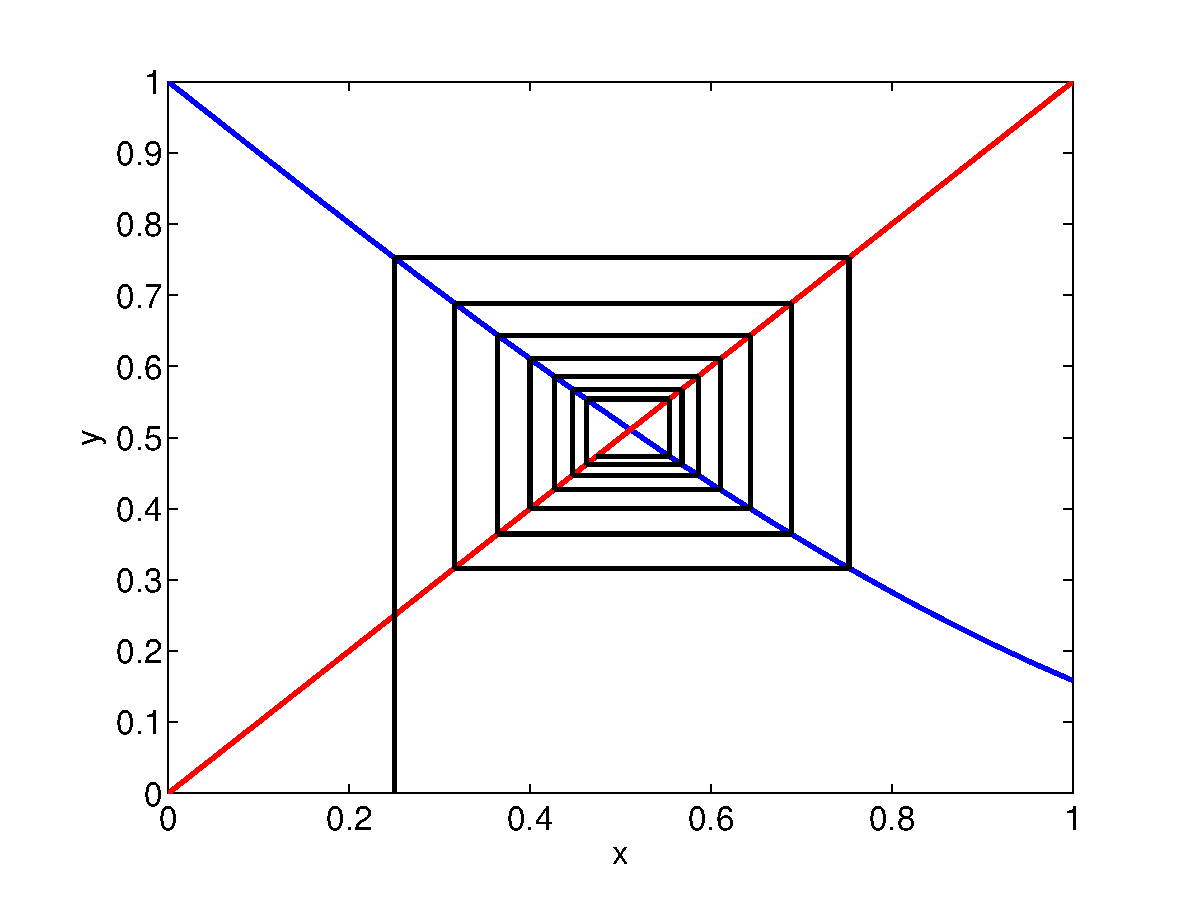
\includegraphics[width=0.7\textwidth]{cobweb_example.eps}
\caption{Example output of \texttt{cobweb} with $g(x) = 1-\sin(x)$ and $x_0 = 0.25$.}\label{fig:cobweb}
\end{figure}
\begin{figure}[p]
\centering
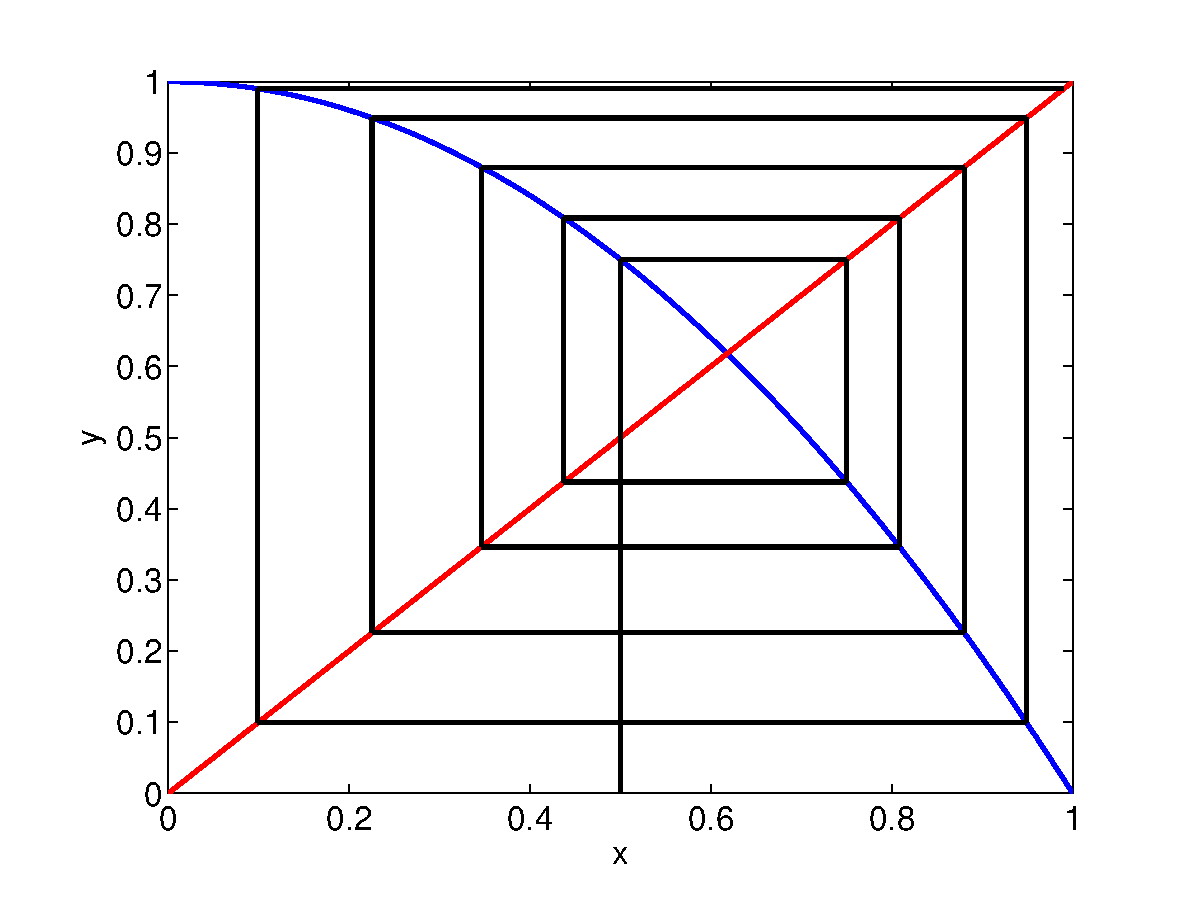
\includegraphics[width=0.7\textwidth]{cobweb_example2.eps}
\caption{Example output of \texttt{cobweb} with $g(x) = 1-x^2$ and $x_0 = 0.5$.}\label{fig:cobweb2}
\end{figure}

\end{questions}

\end{document}
